\section[Проблема в расширении NegativeLiterals]
{Проблема обработки отрицательного нуля в расширении NegativeLiterals}

\subsection{Описание ошибки}

NegativeLiterals решает озвученные проблемы, но, как выяснилось, приносит
новые. Недавно была обнаружена ошибка, связанная с данным расширением.
\cite{trac}

Ошибка заключалась в нераспознавании отрицательного нуля. Без включённого
расширения код \texttt{print (-0::Double)} верно печатал \texttt{-0.0}, но
после включения на экран выводился положительный ноль. Листинг \ref{lst:issue}
это демонстрирует.

\begin{ListingEnv}[H]
\begin{verbatim}
$ ghc-8.0.1 -e '-0.0'
-0.0
$ ghc-8.0.1 -XNegativeLiterals -e '-0.0'
0.0
\end{verbatim}
\caption{Пример ошибки}
\label{lst:issue}
\end{ListingEnv}

rwbarton, обнаруживший данную ошибку, пишет:

\begin{quotation}
Это логично, но неожиданно. Логика такова, что с NegativeLiterals литерал
\texttt{-0.0} обозначает \texttt{fromRational ((-0)\%0)}, что равняется
\texttt{fromRational 0}, что для \texttt{Double} равно положительному нулю,
а не отрицательному.

Но это выглядит неудачно. Возможно, было бы лучше, если \texttt{0.0} (или
\texttt{-} применённый к любому другому литералу математически равному нулю)
был бы рассахарен в \texttt{negate 0.0} даже с NegativeLiterals, так как,
похоже, нет никакой другой причины писать \texttt{-0.0}.
\end{quotation}

\subsection{Первая идея}

Учитывая, что расширение затрагивало только лексический анализатор, мы решили
начать с него. Поведение компилятора с выключенным расширением было правильным,
поэтому мы попробовали модифицировать его правила таким образом, чтобы
NegativeLiterals не влияло на обработку отрицательного нуля.

\begin{ListingEnv}[H]
\begin{verbatim}
$ascnzdigit = 1-9
@nz_decimal = $decdigit* $ascnzdigit $decdigit*
@nz_floating_point = @nz_decimal \. @decimal @exponent?
                   | @decimal \. @nz_decimal @exponent?
                   | @nz_decimal @exponent
\end{verbatim}
\caption{Новые макро определения}
\end{ListingEnv}

Мы добавили два новых макро определения: для ненулевых целых
(\texttt{@nz\_decimal}) и для ненулвых вещественных
чисел(\texttt{@nz\_floating\_point}).

\begin{ListingEnv}[H]
\begin{verbatim}
-  @negative @decimal
    / { ifExtension negativeLiteralsEnabled }
    { tok_num negative 1 1 decimal }
+  @negative @nz_decimal
    / { ifExtension negativeLiteralsEnabled }
    { tok_num negative 1 1 decimal }
...
-  @negative @floating_point
    / { ifExtension negativeLiteralsEnabled }
    { strtoken tok_float }
+  @negative @nz_floating_point
    / { ifExtension negativeLiteralsEnabled }
    { strtoken tok_float }
\end{verbatim}
\caption{Обновлённые правила}
\label{lst:modified-rules}
\end{ListingEnv}

С их помощью мы модифицировали правила расширения NegativeLiterals как показано
в листинге \ref{lst:modified-rules}.

На первый взгляд такое решение работало, что подтверждали простейшие проверки
вроде той, что указана в описании ошибки. К сожалению, запуск тестов выявил
недостатки данного подхода. Листинг \ref{lst:issue-of-solution} демонстрирует,
обнаруженную ошибку.

\begin{ListingEnv}[H]
\begin{lstlisting}
Prelude> print -1
-1
Prelude> print -0
\end{lstlisting}
\begin{verbatim}
<interactive>:2:1:
    Non type-variable argument in the constraint:
                                Num (a -> IO ())
    (Use FlexibleContexts to permit this)
    When checking that ‘it’ has the inferred type
      it :: forall a. (Num (a -> IO ()), Show a)
            => a -> IO ()
\end{verbatim}
\caption{Ошибка}
\label{lst:issue-of-solution}
\end{ListingEnv}

Мы вернули обычное поведение, но забыли, что оно нас не устраивало. В первом
случае минус является частью литерала, а во втором --- отдельной лексемой.
Несмотря на свою простоту такой подход не позволил нам решить проблему, поэтому
необходимо было найти другой способ.

\subsection{Вторая идея}

Решено было отложить обработку отрицательного нуля до более позднего этапа
компиляции. Идея заключалась в том, чтобы для отрицательного нуля генерировать
вызов \texttt{negate}. Для этого понадобилось отдельно от значения литерала
сохранять его знак. Это связано с тем, что значения хранятся в типах
\texttt{Integer} и \texttt{Rational}, в которых нет отдельного значения для
отрицательного нуля.

\begin{ListingEnv}[H]
\begin{lstlisting}
data Token =
...
-  | ITinteger  SourceText Integer
+  | ITinteger  IntegralLit
   | ITrational FractionalLit
...
\end{lstlisting}
\caption{Определения лексем}
\end{ListingEnv}

\begin{ListingEnv}[H]
\begin{lstlisting}
+data IntegralLit
+  = IL { il_text :: SourceText
+       , il_neg :: Bool -- See Note [Negative zero]
+       , il_value :: Integer
+       }
+  deriving (Data, Show)
data FractionalLit
-  = FL { fl_text :: String     -- How the value was written
-                               -- in the source
+  = FL { fl_text :: SourceText -- How the value was written
+                               -- in the source
+       , fl_neg :: Bool        -- See Note [Negative zero]
        , fl_value :: Rational  -- Numeric value of the literal
        }
   deriving (Data, Show)
\end{lstlisting}
\caption{Хранимая в литерале информация}
\end{ListingEnv}

Мы добавили поле \texttt{neg} типа \texttt{Bool} в структуры, хранящие
информацию о литерале. Для отрицательных литералов его значение \texttt{True},
а для положительных \texttt{False}.

На этапе разрешения имён эта информация может быть использована для того, чтобы
обнаружить отрицательный ноль. Идеальным местом для этого оказалась функция
\texttt{rnOverLit}, которая производит разрешение имён перегруженных литералов,
к которым как раз относятся целые и вещественные литералы. В листинге
\ref{lst:rnoverlit} показаны осуществлённые изменения.  Теперь она помимо
литерала возвращает также функцию \texttt{negate}, если она применена к
отрицательному нулю. Это позволяет в любом месте вызова этой функции легко
вставить вызов функции \texttt{negate}.  Может показаться более выгодным
изменить сигнатуру функции \texttt{rnOverLit} так, чтобы она возвращала не
обязательно литерал, а, к примеру, выражение --- уже применённую функцию
\texttt{negate}. К сожалению, существующая кодовая база не позволяла легко
произвести подобное изменение.

\begin{ListingEnv}[H]
\begin{lstlisting}
+isNegativeZeroOverLit :: HsOverLit t -> Bool
+isNegativeZeroOverLit lit
+ = case ol_val lit of
+        HsIntegral i   -> 0 == il_value i && il_neg i
+        HsFractional f -> 0 == fl_value f && fl_neg f
+        _              -> False
+
-rnOverLit :: HsOverLit t -> RnM (HsOverLit Name, FreeVars)
+rnOverLit :: HsOverLit t ->
+             RnM ((HsOverLit Name, Maybe (HsExpr Name)), FreeVars)
 rnOverLit origLit
   = do  { opt_NumDecimals <- xoptM LangExt.NumDecimals
         ; let { lit@(OverLit {ol_val=val})
             | opt_NumDecimals = origLit {ol_val =
                    generalizeOverLitVal (ol_val origLit)}
             | otherwise       = origLit
           }
         ; let std_name = hsOverLitName val
-        ; (SyntaxExpr { syn_expr = from_thing_name }, fvs)
+        ; (SyntaxExpr { syn_expr = from_thing_name }, fvs1)
             <- lookupSyntaxName std_name
         ; let rebindable = case from_thing_name of
                                 HsVar (L _ v) -> v /= std_name
                                 _             -> panic "rnOverLit"
-        ; return (lit { ol_witness = from_thing_name
-                      , ol_rebindable = rebindable
-                      , ol_type = placeHolderType }, fvs) }
+        ; let lit' = lit { ol_witness = from_thing_name
+                         , ol_rebindable = rebindable
+                         , ol_type = placeHolderType }
+        ; if isNegativeZeroOverLit lit'
+          then do { (SyntaxExpr { syn_expr = negate_name }, fvs2)
+                      <- lookupSyntaxName negateName
+                  ; return ((lit' { ol_val = negateOverLitVal val }
+                            , Just negate_name)
+                           , fvs1 `plusFV` fvs2) }
+          else return ((lit', Nothing), fvs1) }
\end{lstlisting}
\caption{rnOverLit}
\label{lst:rnoverlit}
\end{ListingEnv}

Основным местом использования \texttt{rnOverLit} служит функция
\texttt{rnExpr}. В листинге \ref{lst:rnexpr} показано, как мы генерируем
применение функции \texttt{negate} для отрицательного нуля.

\begin{ListingEnv}[H]
\begin{lstlisting}
rnExpr (HsOverLit lit)
-  = do { (lit', fvs) <- rnOverLit lit
-       ; return (HsOverLit lit', fvs) }
+  = do { ((lit', mb_neg), fvs) <- rnOverLit lit
+                                   -- See note: [Negative zero]
+       ; case mb_neg of
+           Nothing -> return (HsOverLit lit', fvs)
+           Just neg -> return ( HsApp (noLoc neg)
+                                      (noLoc (HsOverLit lit'))
+                              , fvs ) }
\end{lstlisting}
\caption{rnExpr}
\label{lst:rnexpr}
\end{ListingEnv}

Сложные изменения в коде требуют развернутого комментария. Для того чтобы
другой программист, работающий с этим кодом, понял почему он написан именно
так, мы написали такой комментарий и добавили ссылки на него в самых важных
местах:

\begin{quote}
\begin{verbatim}
{-
Note [Negative zero]
~~~~~~~~~~~~~~~~~~~~~~~~~
There were problems with negative zero in conjunction
with Negative Literals extension. Numeric literal
value is contained in Integer and Rational types
inside IntegralLit and FractionalLit. These types
cannot represent negative zero value. So we had to
add explicit field 'neg' which would hold information
about literal sign. Here in rnOverLit we use it to
detect negative zeroes and in this case return not
only literal itself but also negateName so that users
can apply it explicitly. In this case it stays
negative zero.  Trac \#13211
-}
\end{verbatim}
\end{quote}

Каждая ошибка, обнаруженная в компиляторе, нуждается в тесте. Мы написали
тест, который способен обнаружить решаемую нами проблему. Он приведён в
листинге \ref{lst:test}.

\begin{ListingEnv}[H]
\begin{lstlisting}
-- | Test for @NegativeLiterals@ extension (see GHC #13211)

{-# LANGUAGE NegativeLiterals #-}

floatZero0 = 0 :: Float
floatZero1 = 0.0 :: Float

floatNegZero0 = -0 :: Float
floatNegZero1 = -0.0 :: Float

doubleZero0 = 0 :: Double
doubleZero1 = 0.0 :: Double

doubleNegZero0 = -0 :: Double
doubleNegZero1 = -0.0 :: Double

main = do
    print (isNegativeZero floatZero0)
    print (isNegativeZero floatZero1)
    print (isNegativeZero floatNegZero0)
    print (isNegativeZero floatNegZero1)
    print (isNegativeZero doubleZero0)
    print (isNegativeZero doubleZero1)
    print (isNegativeZero doubleNegZero0)
    print (isNegativeZero doubleNegZero1)
\end{lstlisting}
\caption{Тест обработки отрицательного нуля}
\label{lst:test}
\end{ListingEnv}

После исправления мелких недочётов и форматирования отладочного вывода все
тесты были пройдены.

\begin{figure}[H]
\centering
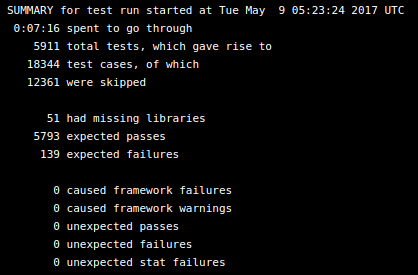
\includegraphics[scale=1]{pic-tests}
\caption{Результаты тестов}
\end{figure}

Для упрощения анализа изменений, вносимых в компилятор, и быстрого прогона
тестов разработчики GHC используют систему Phabricator. Мы опубликовали
изменения с помощью этой системы. \cite{phabricator} Бен Гамари, один из
рецензентов, проанализировал код и согласился принять данные изменения в
основной репозиторий. Это произошло 9 мая \cite{commit}, что поставило точку в
решении проблемы обработки отрицательного нуля.
